\chapter{并行总体方案设计}
\label{cha:chap03}
%基于DTW距离度量的Shapelet
%第二章,第三章介绍了GPU/CUDA并行原理、并行的难点,本章在前面介绍Shapelet和GPU/CUDA相关技术的基础上,提出了基于DTW距离度量的Shapelet并行算法。

%本章首先~\ref{cha:chap04:myalg:Overview}介绍基于DTW距离度量的Shapelet并行算法总体流程、并行方案,整个流程主要按照定义~\ref{def:chap03:Threephases}的三个阶段来执行的:距离计算阶段(~\ref{cha:chap04:myalg:DTW},~\ref{cha:chap04:myalg:euclid})、最佳分割点计算阶段(~\ref{cha:chap04:myalg:infogain})、候选序列筛选阶段。

%第二章介绍了Shapelet的主要流程以及相关工作和GPU/CUDA并行相关原理和技术。

本章首先对于Shapelet调用的相似度/距离度量方法进行了评价和选择,并根据相似度/距离度量方法将距离计算阶段分为两个:w>0距离计算阶段并行方案和w=0距离计算阶段并行方案。然后叙述了基于DTW距离度量的Shapelet并行的总体方案,并对如何根据参数选择执行和各模块的详细功能进行了描述。最后对于并行需要解决的问题进行了识别和解决,比如数据集不断增大问题,特定需求的矩阵转置,最佳分割点计算阶段执行时间长的问题。


%本章是在Shapelet和GPU/CUDA的基础上设计了基于DTW距离度量的Shapelet并行总体方案,并对并行中的一些关键问题进行了识别和解决。

\section{总体方案}
\label{cha:chap04:myalg:Overview}

总体方案章节首先对于Shapelet依赖的相似度/距离计算进行了评价和选择,选择出合适的相似度/距离度量;然后对于总体方案进行叙述,并且对于数据流向以及数据流向和参数的关系进行详细介绍;最后对于总体方案中各模块的职能进行了简单介绍,部分并行模块的职能会在第四章介绍。

%将Shapelet计算过程划分为三阶段,;

\subsection{相似度度量选择}

在章节~\ref{cha:chap02:Distance}介绍各种相似度/距离以及存在的联系。本章节需要选出适用的相似度/距离计算作为Shapelet的相似度/距离调用子程序。

欧式距离$Euclid(A,B)$是Shapelet原始算法的相似度/距离度量,是时间序列数据挖掘应用上有很健壮的性能指标。欧式距离相比其他距离度量的优势在于时间复杂度低,但由于欧氏距离是锁步距离,要求序列上的元素一一对应。

DTW距离$DTW(A,B,w)$容许时间序列进行一定局部延长和压缩,能够克服欧氏距离由于时间序列发生扭曲而无法进行匹配的问题。时间复杂度为$O(wM)$,这里$w$作为控制时间序列扭曲程度一个参数,一般比较小,因为只有时间序列过度扭曲才需要很大的限制区域(即$w$很大)来包含时间序列之间的规整路径,因此,$DTW(A,B,w)$中$w$一般取值为$\left[ 0,C\right),s.t. C << M $,时间复杂度仍为线性。章节~\ref{chap02:euclid2Dtw}对于欧氏距离和DTW关系进行了介绍,欧式距离是DTW的特殊形式,$DTW(A,B,w)\leq DTW(A,B,w=0) = Euclid(A,B)$,使用$DTW(A,B,w)$作为相似度/距离调用在保持欧式距离的健壮性基础上,可以使时间序列进行一定扭曲来进行匹配。

EDR需要提前确定一个超参数$\epsilon$或者对于$EDR(A,B)$中$A,B$进行标准化,所以不适合作为Shapelet作为相似度/距离调用。

综上所述,本文选择$DTW(A,B,w),w\in \left[0,C\right),s.t. C << M$作为Shapelet的相似度/距离度量。当$w>0$时,距离计算阶段采用的距离度量是$DTW(A,B,w)$;而当$w=0$时,为了避免不必要的计算,距离计算阶段采用$DTW(A,B,w)$距离度量的等价方案$Euclid(A,B)$。因此,距离计算阶段会根据$w$的不同分为:w>0距离计算阶段和w=0距离计算级阶段。

\subsection{并行方案}
\label{cha:chap04:myalg:Overview:overallScheme}

\begin{figure}[H] % use float package if you want it here
	\centering
	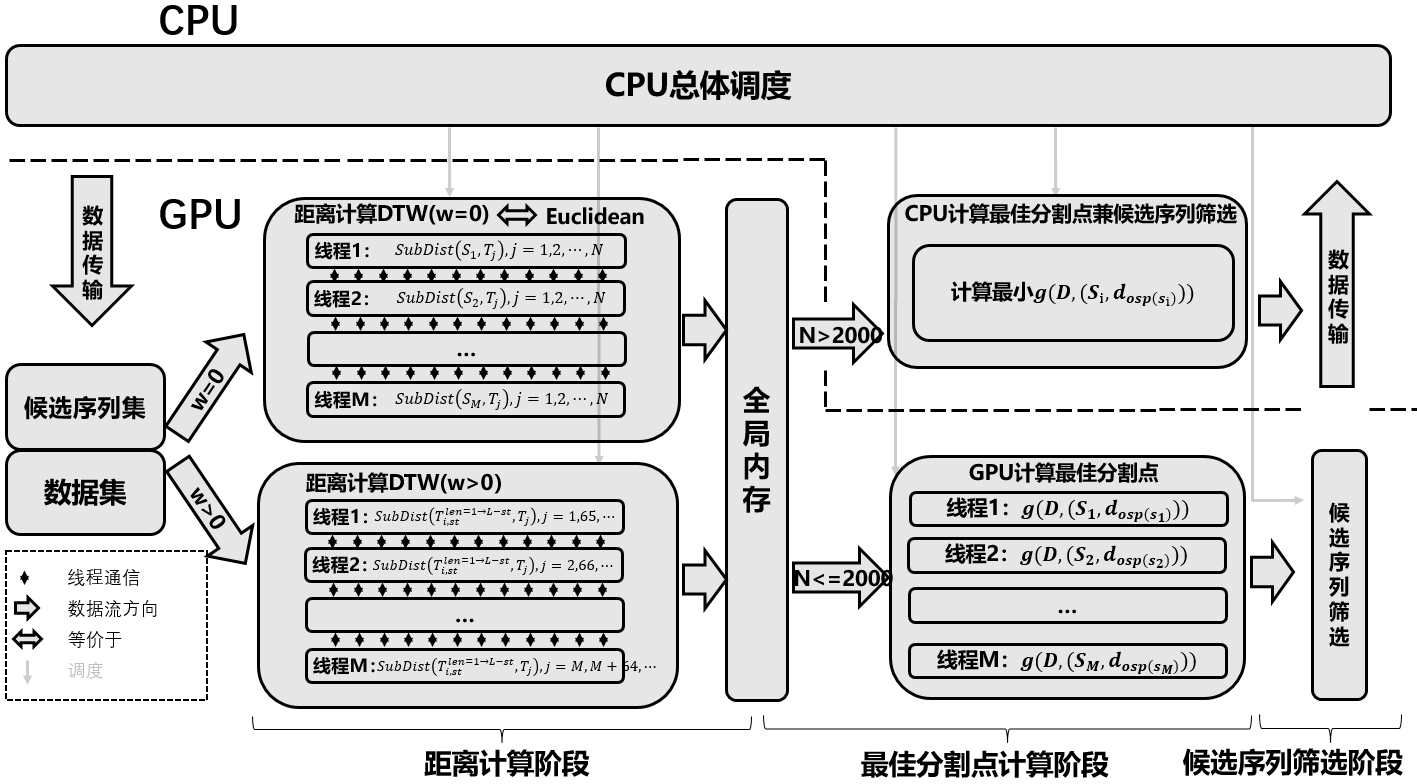
\includegraphics[height=8.3cm]{generalflowchart.png}
	\caption{Shapelet并行总体架构图}
	\label{fig:generalflow}
\end{figure}

图~\ref{fig:generalflow}基于DTW距离度量的Shapelet并行算法的总体架构图,整个并行流程整体符合CPU调度,GPU执行数据计算部分的整体框架,但是数据计算部分会根据数据和参数的不同会有不同的分支处理。数据计算部分主要分为三个阶段:距离计算阶段、最佳分割点计算阶段、候选序列筛选阶段。

1.距离计算阶段:输入候选序列集$S$和数据集$D$,输出多个$\mathcal{F}$并且存储在全局内存中(见定义~\ref{def:chap2:SubDist},公式~\ref{equ:chap2:SubDistSet})。 

2.最佳分割点计算阶段:输入多个$\mathcal{F}$(从全局内存读入),输出信息增益$g(D,(S,d_{osp(S)}))$以及对应的$S$,$d_{osp(S)}$。

3.候选序列筛选阶段:输入多个候选序列$S$以及对应的信息增益$g(D,(S,d_{osp(S)}))$,最佳分割点$d_{osp(S)}$,输出具有最大信息增益的$S$以及对应的$d_{osp(S)}$。

数据计算部分主要有五个模块,分别是w>0距离计算阶段、w=0距离计算级阶段、GPU最佳分割点计算阶段、CPU计算最佳分割点阶段、候选序列筛选阶段,其中CPU计算最佳分割点阶段是在CPU中执行,其他都是在GPU中执行,各模块的只能会在章节~\ref{cha:chap03:modelduty}介绍。

数据计算分布存在较多的分支和参数选择,并行过程会根据数据集的不同和$w$参数的不同选择不同的计算方案,具体数据流向在章节~\ref{cha:chap03:parachoose}介绍。

\subsection{数据流向和参数选择}
\label{cha:chap03:parachoose}

$w$的取值是控制扭曲匹配程度的参数,当$w>0$时,距离计算阶段采用的距离度量是$DTW(A,B,w)$;而当$w=0$时,为了避免不必要的计算,距离计算阶段采用$DTW(A,B,w)$距离度量的等价方案$Euclid(A,B)$。因此,距离计算阶段会根据$w$的不同分为:w>0距离计算阶段和w=0距离计算级阶段。另外,一个Block中最多出现1024个线程,$w=0$距离计算阶段允许最长的时间序列长度$L$为1024。

因此,当$w>0$或$L>1024$时,执行w>0距离计算阶段算法,距离度量采用$DTW(A,B,w)$;而当$w=0$且$L<=1024$时,距离度量采用$DTW(A,B,w=0)$的等价方案$Euclid(A,B)$,执行w=0距离计算阶段算法。

GPU上多线程计算最佳分割点,每个线程需要$O(N)$的空间,但是硬件环境每个Block只能提供48K的共享内存和64K的寄存器大小(见表~\ref{tab:gpuversion}),可能会出现内存不足或者过大内存需求导致每个SM上运行的Warp个数减小。虽然通过调节Block的参数能够一定程度上缓解这种情况,但是依然存在这样一个阈值,当$N$大于这个阈值时,GPU将不能提供足够的资源进行最佳分割点并行计算。因此,设定一个阈值$N_{th}=2000$(根据一个$block$执行32个线程所需资源计算),当$N\leq N_{th}$时,最佳分割点计算时,会在GPU中执行;当$N>N_{th}$时,最佳分割点计算会在CPU中执行,其中CPU和GPU执行最佳分割点的算法相同。

因为CPU计算最佳分割点是通过将共享内存中的$\mathcal{F}$拷贝到主机中然后串行执行的,因此CPU计算最佳分割点对应的候选序列筛选可以通过串行的方法一并进行。

对于w>0距离计算阶段、w=0距离计算级阶段、最佳分割点计算阶段,会估计不同数据集即不同$w,N,L$参数下每个$Block$中共享内存和寄存器的使用情况。本文对于不同的$w,N,L$设置了资源使用上线,会根据不同的参数调节$Block$和$Grid$参数,避免单个Warp占用资源太多,而影响SM上同时执行的Warp个数,这样可以使有限的资源上进行更多的计算。
%
%整个并行执行流程会根据$w,N,L$的不同选择不同的执行路径,在保证完成计算和内存需要的基础上,尽可能进行更多的计算。

\subsection{各模块职能}
\label{cha:chap03:modelduty}
%
%整个并行流程整体符合CPU调度,GPU执行数据计算部分的整体框架,但是数据计算部分会根据数据和参数的不同会有不同的分支处理。数据计算部分主要分为三个阶段:距离计算阶段、最佳分割点计算阶段、候选序列筛选阶段。
本章节主要介绍并行框架中的五个模块和全局内存的职能,这五个模块包括w>0距离计算阶段、w=0距离计算级阶段、GPU最佳分割点计算阶段、CPU计算最佳分割点阶段、候选序列筛选阶段

%\textbf{距离计算阶段}:在GPU中计算每个候选序列$S$对于数据集$D$每个时间序列$T_j$的距离$SubDist(S,T_j),j=1,2,\cdots,N$,然后存储在全局内存中。这一部分计算会根据$N,L,w$选择不同的计算方式:距离计算阶段按照$w$或者$L$取值的不同分为$w>0$距离计算阶段和$w=0$距离计算阶段;$N$的大小主要影响距离计算阶段的Block参数选择,选用占有率最高的方案,从而到达执行效率最高,这一点本文不做详述。

\textbf{全局内存}:全局内存承担距离计算阶段和最佳分割点计算阶段的中间媒介,距离计算阶段将距离计算结果$\mathcal{F}$存入全局内存,最佳分割点计算阶段再从全局内存读取$\mathcal{F}$来计算最佳分割点,其中距离计算阶段和最佳分割点计算阶段都使用全局内存访问的方法,从而减少全局内存访存延时。

\textbf{w>0距离计算阶段算法}:距离度量采用$DTW(A,B,w)$,每个线程主要负责$T_i$中以$s$位置为起始的所有候选序列$\left\lbrace T_{i,s}^{len},len=1\to L-s\right\rbrace $和数据集中几个时间序列$T_j$的距离计算,如公式~\ref{equ:chap04:everythread2},具体实现细节会在章节~\ref{cha:chap04:myalg:DTW}介绍。
%\begin{equation}
%\label{equ:chap04:everythread2}
%\begin{array}{l}
%SubDist(T_{i,s}^{len},T_j), \\ [0.3cm]
%s.t.~ len=1\to(L-s),j=\left\lbrace tid_x,tid_x+dim_{tidx},tid+2*dim_{tidx},\cdots \right\rbrace  
%\end{array}
%\end{equation}
\begin{equation}\label{equ:chap04:everythread2}
\left\{\begin{array}{l}
\left\lbrace SubDist(T_{i,s}^{len},T_j) \right\rbrace \\[0.1cm]
\mbox{subject to:}\\[0.1cm]
\qquad len=1\to (L-s)\\[0.1cm]
\qquad j=\left\lbrace tid_x,tid_x+dim_{tidx},tid+2*dim_{tidx}\right\rbrace 
\end{array}\right.
\end{equation}

\textbf{w=0距离计算阶段算法}:距离度量采用$Euclid(A,B)$,每个线程执行一个候选序列$S$相对于数据集$D$所有时间序列$T_j$计算距离$SubDist(S,T_j),j=1\to N$。一个Block中多个线程的候选序列是一个时间序列的长度为$len$的子序列,比如$Block(i,len)$计算候选序列就是$T_{i,s}^{len},s=1,2,\cdots,L-len+1$。$w=0$距离计算阶段算法中线程存在依赖关系,需要线程之间进行协作计算,详见章节~\ref{cha:chap04:myalg:euclid}。

\textbf{GPU最佳分割点计算阶段}:这一阶段会从全局内存读取$\mathcal{F}$吗,然后并行计算出对应的最佳分割点$d_{osp}$,这里使用了启发式算法计算最佳分割点,详细设计见章节~\ref{cha:chap04:myalg:infogain}。这一阶段会根据不同$N$大小使用不同的共享内存及寄存器改变相应的$grid$和$block$参数,使尽可能多的线程同时并行计算。

\textbf{CPU最佳分割点计算阶段}采用的算法和GPU计算最佳分割点的算法是相同的,不同的是在CPU中执行。当N增大到一定程度时,SM上的资源不再足够32个线程执行,就会切换到CPU执行。

\textbf{候选序列筛选阶段}:最佳分割点阶段产生$O(NL^2)$个候选序列$S$及其对应的信息增益$g(D,(S,d_{osp(S)}))$和分割点$d_{dsp(S)}$,在本阶段需要选出具有最大信息增益的候选序列及其对应的分割点。这一阶段的本质是一个特大向量求最大值的过程,是一个典型的归约过程,可以采用并行归约的算法求最大信息增益,时间复杂度为$O(\log(N)+\log(L))$。我们这里并没有直接使用归约算法,而是将原始归约算法~\cite{harris2007optimizing}的求最大值过程改造成求最大值索引过程,这样能够避免候选序列和分割点跟随信息增益一起归约。因为并行求最大信息增益过程总的时间占比不超过1\%,本文不做过多的介绍。另外,正因为候选序列筛选阶段是一个归约过程,为了保持高效率,使用独立的并行计算完成。

%因为需要规约计算筛选候选序列的原因,
%至于从信息增益处又分为两个阶段的原因,并行计算最佳分割点阶段必然产生大量候选序列$S$以及对应的信息增益$g(D,(S,d_{osp(S)}))$和分割点$d_{osp(S)}$。求最大信息增益的过程相当于一个向量求最大值的过程,可以使用归约的算法迅速完成$O(NL^2)$个候选序列的筛选,放在GPU中的时间复杂度时间$O(\log(N)+\log(L)$,最后GPU和主机之间只需要拷贝一次候选序列筛选的结果$Shapelet(D)$以及对应的分割点。相反如果直接放在CPU阶段计算会存在一次空间大小$O(NL^2)$的GPU和设备之间的内存拷贝和$O(NL^2)$时间复杂度的最大值计算,$O(NL^2)$的空间复杂度和时间复杂度对于本算法不是很明显,当数据集很大时,还是很耗时间的。为了尽量减少执行时间,将定义~\ref{def:choose}过程放在GPU中执行,这里称为求最大信息增益阶段。

%距离计算阶段:在GPU中计算每个候选序列$S$对于数据集$D$每个时间序列$T_j$的距离$SubDist(S,T_j),j=1,2,\cdots,N$,然后存储在全局内存中(global Memory)。这一部分计算会根据$N,L,w$选择不同的计算方式:距离计算阶段按照$w$或者$L$取值的不同分为$w>0$距离计算阶段和$w=0$距离计算阶段;$N$的大小主要影响距离计算阶段的Block参数选择,选用占有率最高的方案,从而到达执行效率最高,这一点本文不做详述。
%计算结果是通过线程协作计算而来,详细设计见章节~\ref{cha:chap04:myalg:euclid}。
%当$w=0$且$L<=1024$时,距离度量采用$DTW(A,B,w=0)$的等价方案$Euclid(A,B)$,因为采用$Euclid(A,B)$更加节省时间(见章节~\ref{chap02:euclid2Dtw})。
%CPU最佳分割点计算阶段:当$N$大于一定值时,最佳分割点计算会在CPU上进行。因为每个线程需要$O(N)$的空间,但是硬件环境每个Block只能提供48K的共享内存和64K的寄存器大小(见表~\ref{tab:gpuversion}),GPU上最佳分割点计算还是右可能会出现内存不能满足的情况,即使调节每个Block的参数,依然有这样一个阈值存在,因此,当$N$大于一定值时,最佳分割点会在CPU上执行。CPU计算最佳分割点是将多个候选序列$S$对应的$\mathcal{F}$从GPU拷贝的主机,在CPU上逐个运行最佳分割点计算并取最小值。
%候选序列$S$对应的$\mathcal{F}$需要$O(N)$的空间复杂度,数据集$D$中有$O(NL^2)$个$\mathcal{F}$,如果一次执行完所有流程,需要使用全局内存空间复杂度至少为$O(N^2L^2)$。
%当数据集比较小时,GPU的全局内存可以满足$O(N^2L^2)$的空间复杂度,一旦数据集大小和时间序列长度增大,GPU很容易导致全局内存不足。为了解决全局内存不足的问题,这里采用换入换出、分段计算的方法进行计算,限制每次计算$\mathcal{F}$最大数量(根据全局内存大小和数据集来确定$\mathcal{F}$个数)。


\section{并行需要解决的问题}

本章节主要介绍设计并行算法之前需要解决的问题,包括数据集不断增大问题、特定需求的矩阵转置、计算最佳分割点的执行时间问题。

\subsection{数据集不断增大的问题}
\label{cha:chap03:Problemsencountered:BigDataSet}

$\mathcal{F}$是计算Shapelet中一个空间复杂度为$O(N)$的中间变量,是计算距离和最佳分割点的中间变量。当数据集大小及时间序列长度$N,L$很小的时候,我们采用寄存器存储$\mathcal{F}$,不会涉及到访存延时,计算速度会很快。

当$N,L$增大时,CUDA会将寄存器存不下的内容放在局部内存中(局部内存实际上占用全局内存空间,和全局存储速度一致,但是又没有使用合并存储器访问,会有很大的访存延时),各线程会出现频繁的访存延时而表现性能非常差。Shapelet并行算法需要计算大量候选序列$S$对应的$\mathcal{F}$,有限的寄存器和共享内存都不能满足$\mathcal{F}$存放的要求,这里我们考虑将$\mathcal{F}$放在全局内存中存储,将$\mathcal{F}$作为作为计算距离和最佳分割点的中间变量。$\mathcal{F}$两个阶段的中间变量,为了保证执行时间,距离计算阶段必须通过Coalesced将$\mathcal{F}$存储到全局内存,最佳分割点计算阶段必须通过Coalesced方式从全局内存读取$\mathcal{F}$。

将$\mathcal{F}$放在全局内存中存储,只能一定程度上解决资源不足的问题。当$N,L$继续增大时,全局内存依旧不能满足$\mathcal{F}$的资源需求。$\mathcal{F}$作为候选序列$S$对于距离计算结果,空间复杂度为$O(N)$,数据集$D$中共有$O(NL^2)$个$S$,
则$\mathcal{F}$共需要$O(N^2L^2)$的空间。随着$N,L$的增大,全局内存肯定不能提供平方级别的空间需求,$O(N^2L^2)$的空间复杂度很快会使内存超过全局内存大小。对于全局内存存储中间结果$\mathcal{F}$空间不足的情况,这里使用数据分割~\cite{li2016data}的思路去解决,每次将候选序列集的某个子集在GPU中使用进行并行计算,再在CPU上综合多次计算的结果,具体如图~\ref{fig:Swapinout}。当然有多块GPU可供使用时,也可以多个GPU同时并行多个候选序列子集,然后再统一归约。这里涉及的分割策略、数据在主机和GPU之间拷贝,不再这里详述。

\begin{figure}[H] % use float package if you want it here
	\centering
	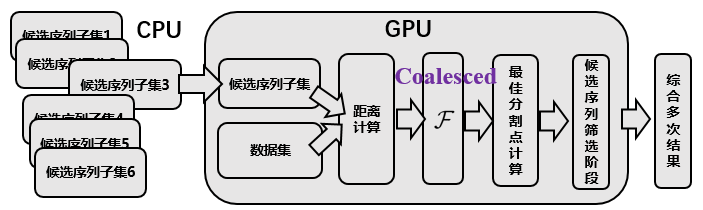
\includegraphics[width=12.2cm]{Swapinout.png}
	\caption{数据集不断增大的解决方案}
	\label{fig:Swapinout}
\end{figure}

这里解释一下为什么从$\mathcal{F}$中间变量处分为距离计算和最佳分割点计算两个阶段,主要三个原因:

1.距离计算阶段和最佳分割点是不同性质的计算,将两者分开更有利于保持各线程均衡,有利于资源的充分利用;

2.在距离计算阶段,后文根据$w$的不同分为$w>0$距离计算阶段和$w=0$距离计算阶段,两者访问$\mathcal{F}$的方式不同;

3.从$\mathcal{F}$处分开有利于算法实现,使每个$kernel$的功能都比较清晰。


\subsection{特定需求的矩阵转置}

在$w=0$距离计算阶段中,每个Block都会产生一个矩阵,我们需要将每一个矩阵中的列向量变成行向量,这时候就需要采用矩阵转置过程。但是这里我们不能使用CUBLAS~\cite{chrzeszczyk2013matrix}中库或者或现成算法,原因有两点:

第一:如图~\ref{fig:customtranspose},每一个Block产生一个$M*N$的矩阵都存储在全局内存一个$C*R$的一个块中,矩阵并没有占据整个块的空间;每个Block产生矩阵列数$M$不一致,但是$C,R$的大小是根据最大的$M,N$确定,而$M$的差别有可能很大,如图~\ref{fig:customtranspose}中的$Block_1$和$Block_2$。调用算法的矩阵转置都是按照$C*R$的大小进行转置的,有可能造成大量计算资源浪费。

第二:我们这里要求转置之后的矩阵行与行之间是拼接起来的,如图~\ref{fig:customtranspose}右侧部分。如果调用现成算法的矩阵转置之后的每个矩阵之间都会出现空白,如果需要按行拼接起来,必须再进行一次全局内存拷贝过程,这样同样违背我们加速的目的。

我们需要设计一个矩阵转置算法能够做到资源合理利用,可以从以下两个角度进行:

1.对于不同大小的矩阵,根据矩阵的实际大小进行转置,转置的大小不能$(M+32,N+32)$;

2.计算每个矩阵转置拼接之后的偏移和行数,方便直接转置到偏移位置。
\begin{figure}[H] % use float package if you want it here
	\centering
	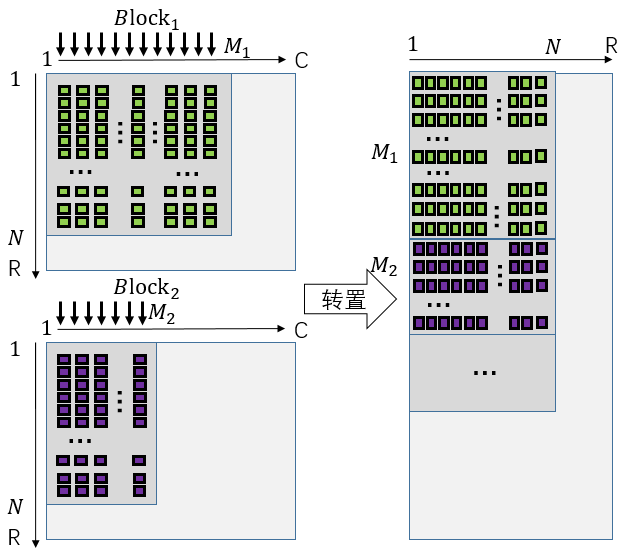
\includegraphics[height=9cm]{customtranspose.png}
	\caption{特定矩阵转置要求}
	\label{fig:customtranspose}
\end{figure}
\subsection{计算最佳分割点的执行时间问题}

距离计算阶段的时间复杂度为$O(N^2L^4)$,距离计算是Shapelet发现复杂度最高的计算。但是距离计算阶段的时间复杂度可以降到$O(N^2L^3)$,最佳分割点计算阶段的时间复杂度为$O(N^2L^2\log(N))$。

当数据集$D$很大时,即$N$很大时,最佳分割点阶段有可能成为Shapelet发现过程占比时间最大的计算。我们需要降低最佳分割点计算的时间复杂度,从而降低执行时间。

传统的最佳分割点计算,对于所有可能的阈值$d_{th}$都进行了尝试,如~\ref{equ:chap3:Infogain}。一般会将$\mathcal{F}$按照距离进行排序(排序时间复杂度$O(N\log(N))$)之后,以每两个距离之间的值作为阈值$d_{th}$进行尝试,这是以一种遍历的方法寻找全局最优值。
\begin{equation}
\label{equ:chap3:Infogain}
	g(D,(S,d_{osp(S)})) \geq g(D,(S,d_{th})),\forall d_{th}\in \mathbb{R}_{+}
\end{equation}

但是我们的目的不是对于距离进行排序,我们是需要找一个阈值$d_{th}$,将数据集$D$中的两类尽可能分开。这里可以采用一种启发式的搜索方法,搜索满足条件的阈值。因为候选序列非常多,可以使用不同的搜索方式来使其中一种候选序列产生的阈值尽量靠近全局最优值。

%\subsection{优化困难}
%
%1024线程与$N$的关系
%不同的数据如何选择不同的算法?
%
%同时跑完
%
%上面提到实现一个并行程序不是很难,但是使并行程序表现出很好的性能需要消耗大量的时间。
%
%比如grid参数考虑
%
%今天想到一个可以放在这里的问题?
%Bank-Conflict 各种参数的计算?
%Share-Mem 在DTW不并行的情况下有可能是没有用的.

\section{本章小结}

%本文首先对于Shapelet调用的相似度度量方法进行了评价和选择,并根据相似度度量方法将距离计算阶段分为两个:w>0距离计算阶段并行方案和w=0距离计算阶段并行方案。然后叙述了基于DTW距离度量的Shapelet并行的总体方案,并对如何执行和各模块功能进行了详细描述。最后对于并行需要解决的问题进行了识别和解决。

%本章首先对于Shapelet调用的相似度度量方法进行了评价和选择,并根据相似度度量方法将距离计算阶段分为两个:w>0距离计算阶段并行方案和w=0距离计算阶段并行方案。然后叙述了基于DTW距离度量的Shapelet并行的总体方案,并对如何根据参数选择执行和各模块的详细功能进行了描述。最后对于并行需要解决的问题进行了识别和解决,比如数据集不断增大问题,特定需求的矩阵转置,最佳分割点计算阶段执行时间长的问题。

总的来说,本章距离选择和评价部分解释了为什么会出现两个距离计算阶段:w>0距离计算阶段并行方案和w=0距离计算阶段并行方案;并行方案部分介绍了基于DTW距离度量的并行Shapelet的总体框架;数据流向和参数选择部分
详述了如何根据数据的特点选择最佳的计算方案即数据流向;各模块内容部分叙述了各个模块的职能,其中并行模块部分介绍了每个线程的职能。
%
%本章首先介了绍基于DTW距离度量的Shapelet并行总体方案设计,然后对各模块的功能进行详细描述,最后对于并行中需要解决的一些关键问题进行了识别和解决。
%本章主要介绍了GPU/CUDA并行相关技术和的Shapelet的并行难点进行解决。首先介绍了GPU的硬件架构以及使用CUDA如何使用硬件环境加速并行的;然后本文使用到的CUDA加速技术,例如合并内存访问、存储体冲突、延时隐藏、Warp分歧等;最后对于本文将要遇到的并行难题进行解决。



